\documentclass[Main]{subfiles}
\begin{document}

\chapter{Hardware}

\section{Hardware oversigt}

Til styring af drone, skulle der laves en sender og en modtager.

\begin{figure}[H]
\centering
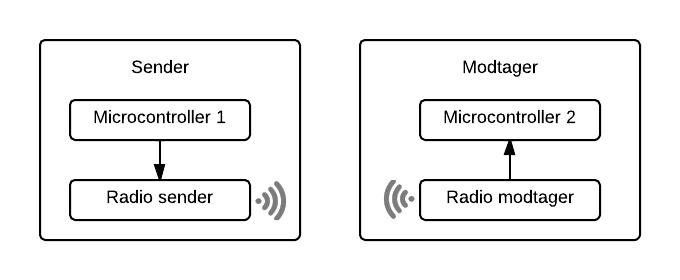
\includegraphics[scale=0.6]{Blokdiagram}
\caption{Skitse af hardware}
\label{Fig:Blokdiagram}
\end{figure}

\code{Sender} enhed som brugeren anvender til system-input.
\code{Modtager} er den enhed der er sat på dronen, som skal modtage brugerens system-input.
Det vil sige der skulle laves to enheder, vist på Figur \ref{Fig:Blokdiagram}.
Radioen er baseret på chippen CC1101\cite{TI-cc1101} fra Texas Instruments. 
µ-Controlleren er en ATmega8\cite{AtmelMega8} fra Atmel Corporation.
\\ \code{Senderen} skal også have knapper så brugeren kan lave sit input.


\newpage
\section{Grænseflader}
De interne og eksterne grænseflader:
\vspace{-20pt}
\begin{itemize}
\item SPI er designet i forhold til Atmels standarter\cite{SPI}.
\item \itoc / TWI er designet i forhold til Atmels standarter \cite{Twi}.
\end{itemize}




\subsection{Sender}
\begin{figure}[H]
\centering
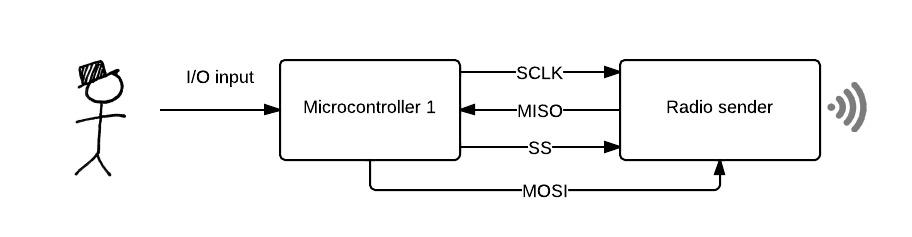
\includegraphics[scale=0.5]{SenderInterface}
\caption{Grænseflader for sender}
\label{fig: SenderInterface}
\end{figure}

På Figur \ref{fig: SenderInterface} ses et blokdiagram af senderen med alle grænseflader.
De eksterne grænseflader er der, hvor brugeren skal lave sit input. Det vil sige der er her han laver et programvalg som bliver sendt videre til dronen.
De interne grænseflader som er kommunikationen mellem µ-controller 1 og radiosenderen, foregår via SPI-protokollen. 

Radio-interfacet er beskrevet i sektionen Radio (Afsnit \ref{Sec:Radio}).



\subsection{Modtager}

\begin{figure}[H]
\centering
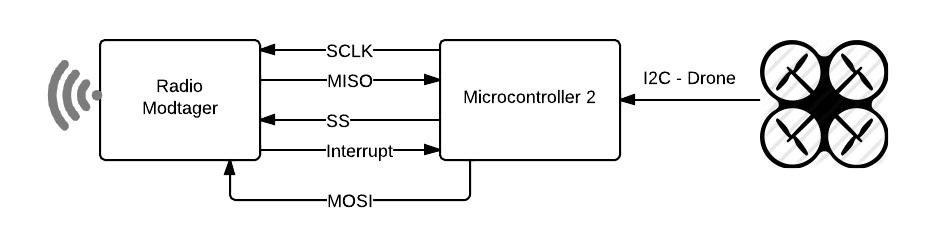
\includegraphics[scale=0.5]{ModtagerInterface}
\caption{Grænseflader for modtager}
\label{fig: ModtagerInterface}
\end{figure}

På Figur \ref{fig: ModtagerInterface} ses et blokdiagram af modtageren med alle grænseflader.
Radioen modtager en pakke fra senderen. Når hele pakken er modtaget udføres et interrupt på µ-controller 2.

µ-Controller 2, henter hele pakken fra radioen og sætter den i modtage-mode igen. 
Den tager så de modtagne data fra radioen og skriver dem i en output buffer til \itoc forbindelsen.

Radio-interfacet er beskrevet i Afsnit \ref{Sec:Radio}.


\subsection{Radio} \label{Sec:Radio}

Opsætningen på radioen som bliver anvendt er som følger:
\vspace{-20pt}
\begin{itemize}
\item 433 MHz radio frekvens.
\item 2.5 kbps overførselshastighed.
\item CRC af dataoverførslen.
\item Benytter kanal 0 i 433 MHz frekvensbåndet.
\end{itemize}


Framet, der bliver sendt frem og tilbage, ser ud som på Figur \ref{fig: Pakke}.

\begin{figure}[H]
\centering
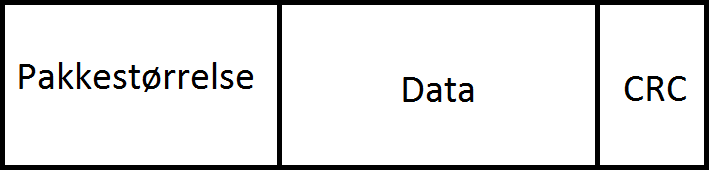
\includegraphics[scale=0.8]{Pakke}
\caption{Framens opbygningen}
\label{fig: Pakke}
\end{figure}

\paragraph{Pakkens opbygning:}\mbox{}\\
Pakkestørrelsen er længden af den samlede pakke, eksklusiv CRC-delen. 
Grunden til denne skal med er, at radioerne er sat op til en variabel pakkestørrelse. 
De kan også sættes til en fast længde, så er der ikke brug for denne.

Dataen er payloaden -- det er her alle de informationer der skal sendes frem og tilbage ligger. 
Det vil sige, at et program er valgt efterfulgt af hvilket program det er.

CRC er en checksum som sendes med. 
Den sikrer at framet der transmitteres ikke er corrupt.



\section{Design}
Det der skulle designes, var et print til sender og et til modtager.

\subsection{Sender}
Senderprintet indeholder knapper, en ATmega8 µ-processorer og en socket til radiosenderen.

Knap-designet er aktivt lav, som det kan ses på Figur \ref{fig: Knapper}.


\begin{figure}[H]
\centering
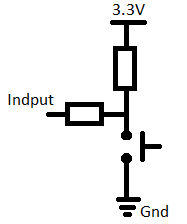
\includegraphics[scale=0.8]{Knapper}
\caption{Design af knapper}
\label{fig: Knapper}
\end{figure}

Der er 9 knapper (Tach Switchs) i alt, til styring af dronen.\\
Skematic af hele senderen kan ses i Bilag\cite{SenderSCM}.


\subsection{Modtager}

Modtagerprintet indeholder en ATmega8 µ-controller og en radiosender.

Dette design indeholder en socket til radioen og en socket til \itoc-forbindelsen til dronen.
Skematic af systemet kan ses i Bilag\cite{ModtagerSCM}.


\subsection{Strøm input}

Senderen og modtageren kører på 3.3 V.
Der er ikke lavet noget beskyttelse på spændingsinputtet, så de 3.3 V (DC) skal være præcis.

Det totale strømforbrug for hele sender systemet er:
\vspace{-20pt}
\begin{itemize}
\item 8 mA passiv, dvs. når der ikke sendes.
\item 43 mA aktiv, dvs. når der trykkes på en knap så data sendes til modtager.
\end{itemize}

Så det vil sige at senderen på et AA 2000 mA batteri kan være på standby i $\dfrac{2000 \frac mA\cdot h}{8 mA} = 250 h$ eller sende i $\dfrac{2000 mA \cdot h}{43 mA} = 46,5 h$.


\newpage
\section{PCB layout}

\begin{figure}[H]
\centering
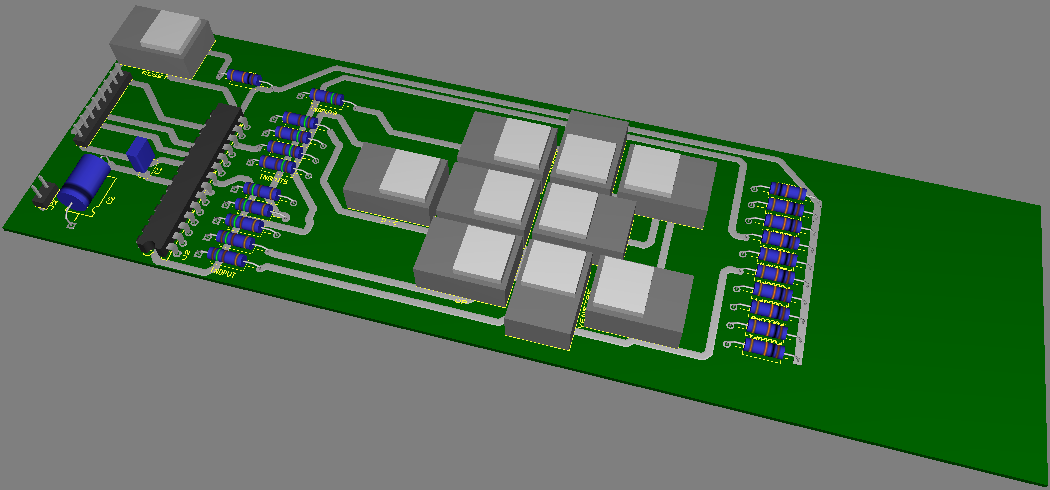
\includegraphics[scale=0.5]{Print3D}
\caption{Det færdige print}
\label{fig: Print3D}
\end{figure}

Det endelige layout kan ses på Figur \ref{fig: Print3D}.
Layoutet er forsøgt holdt simpelt. 
Knapperne til brugeren er placeret så de minder om pilene på et tastatur, dog med op/ned funktioner og autoland.
Printet er aflangt, så det er til at holde som en fjernbetjening og derved kan styres med én hånd.
Radioen er placeret forrest på fjernbetjeningen, for at brugeren dæmper/skærmer mindst muligt for signalet.  


\newpage
\section{Sonar-klods}\label{Sec:Sonar}
På dronens frontben sidder en lille klods, som holder sonarsensorerne.
Da benet er har en skæv vinkel til dronen og sensorerne gerne skal være lodrette, er klodsen skåret i en skæv vinkel.
Derudover peger hver sensor således, at deres bølger først overlapper hinanden efter 50 cm. 
Hver sensor spreder sig over $67^\circ$ (se Figur \ref{Fig:SonarMeasure}), hvilket gør, at klodsen skal skæres til $32^\circ$ til hver side, vist på Figur \ref{Fig:SonarSkitse}.
\begin{figure}[H]
\centering
	\begin{subfigure}[b]{0.45\textwidth}
		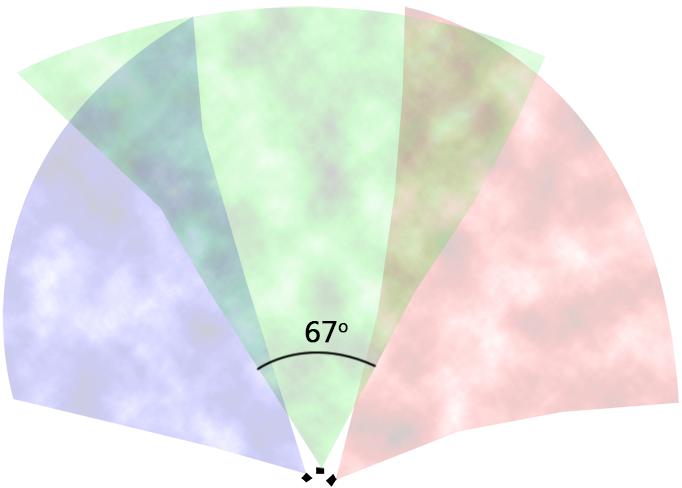
\includegraphics[width = \textwidth]{SonarOverlap}
		\caption{Måling af sonarspredning}
		\label{Fig:SonarMeasure}
	\end{subfigure}
	\quad
	\begin{subfigure}[b]{0.45\textwidth}
	\centering
		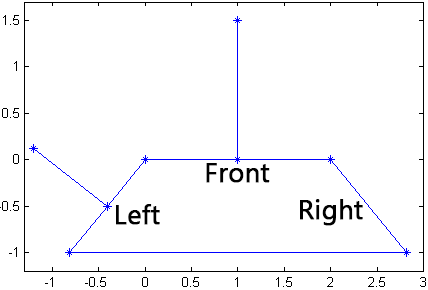
\includegraphics[width =\textwidth]{Sonar}
		\caption{Sonarklods-skitse. Beregningerne kan ses i bilag\cite{Klods}}
		\label{Fig:SonarSkitse}
	\end{subfigure}
	\caption{Sonar spektrum og skitse.}
\end{figure}

Sensorerne er programmeret til, at give en advarsel hvis de registrerer noget inden for 100 cm.
Sensorerne bliver dog først aktiveret, når dronen selv skal holde styr på sin højde. Dette skyldes, at de udsender deres bøljer i en kegle, og ikke kun horisontalt. 
Det betyder, at dronen vil kunne se jorden under den, såfremt den flyver lavt nok (eller den i opstartsfasen står på jorden).

\begin{figure}[H]
\centering
	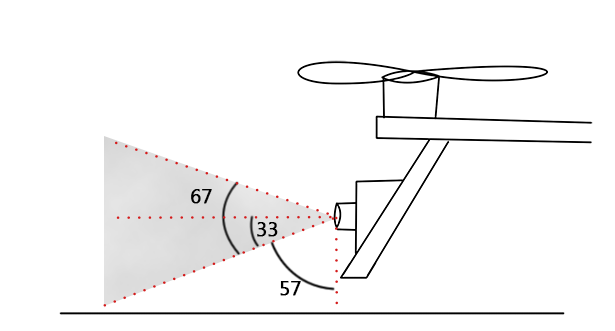
\includegraphics[width = 0.7 \textwidth]{SonarAngles}
	\caption{Sonarsensorernes afstand til jorden}
	\label{Fig:SonarAngles}
\end{figure}

Fra sensoren til nærmeste forhindring er der maksimalt 100 cm, og da gulvet ikke skal rammes skal der holdes en hvis afstand hertil.
\vspace{-10 pt}
\begin{align*}
%b &= \dfrac{sin(B) \cdot c}{sin(C)} & \text{Afstanden på jorden} \\
%	&= \dfrac{sin(57) \cdot 100}{sin(90)} = 83.87 \\
A &= 180^\circ - C - B & \text{Vinklen fra jorden til sensoren}\\
	&= 180^\circ - 90^\circ - 57^\circ\\
	&= 33 ^\circ\\
a &= \dfrac{sin(A) \cdot c}{sin(C)} & \text{Afstanden fra sonar til jorden}\\
 	&= \dfrac{sin(33^\circ) \cdot 100cm}{sin(90^\circ)} \\
	&= 54.46 cm
\end{align*}
Der skal altså være minimum 55 cm fra dronen til jorden, før dette har en effekt.







\end{document}
